\documentclass[border=6pt]{standalone}
% Shared draw.io-matching colours and node styles for the thesis flowcharts.
\usepackage{tikz}
\usetikzlibrary{shapes.geometric, arrows.meta, positioning, calc}

% Keep words whole inside boxes (no ugly mid-word hyphenation)
\hyphenpenalty=10000\exhyphenpenalty=10000\tolerance=2000

% draw.io standard palette (fill + stroke)
\definecolor{dioBlueF}{HTML}{DAE8FC}\definecolor{dioBlueS}{HTML}{6C8EBF}
\definecolor{dioOrangeF}{HTML}{FFE6CC}\definecolor{dioOrangeS}{HTML}{D79B00}
\definecolor{dioGrayF}{HTML}{F5F5F5}\definecolor{dioGrayS}{HTML}{666666}
\definecolor{dioGreenF}{HTML}{D5E8D4}\definecolor{dioGreenS}{HTML}{82B366}
\definecolor{dioPurpleF}{HTML}{E1D5E7}\definecolor{dioPurpleS}{HTML}{9673A6}

\tikzset{
  >={Stealth[length=2.4mm]},
  fnode/.style={rounded corners=5pt, draw, line width=0.8pt,
    minimum width=2.7cm, minimum height=1.15cm, align=center,
    font=\small, text width=2.5cm, inner sep=2pt},
  blue/.style ={fnode, fill=dioBlueF,   draw=dioBlueS},
  orange/.style={fnode, fill=dioOrangeF, draw=dioOrangeS},
  gray/.style ={fnode, fill=dioGrayF,   draw=dioGrayS},
  green/.style={fnode, fill=dioGreenF,  draw=dioGreenS},
  purple/.style={fnode, fill=dioPurpleF, draw=dioPurpleS},
  decision/.style={diamond, draw, line width=0.8pt, aspect=1.7,
    align=center, font=\small, text width=1.9cm, inner sep=0pt,
    fill=dioGrayF, draw=dioGrayS, minimum width=3cm, minimum height=2.3cm},
  bdecision/.style={decision, fill=dioBlueF, draw=dioBlueS},
  flow/.style={->, line width=0.8pt, draw=black!75},
  elabel/.style={font=\footnotesize, inner sep=1.5pt, fill=white},
}

\begin{document}
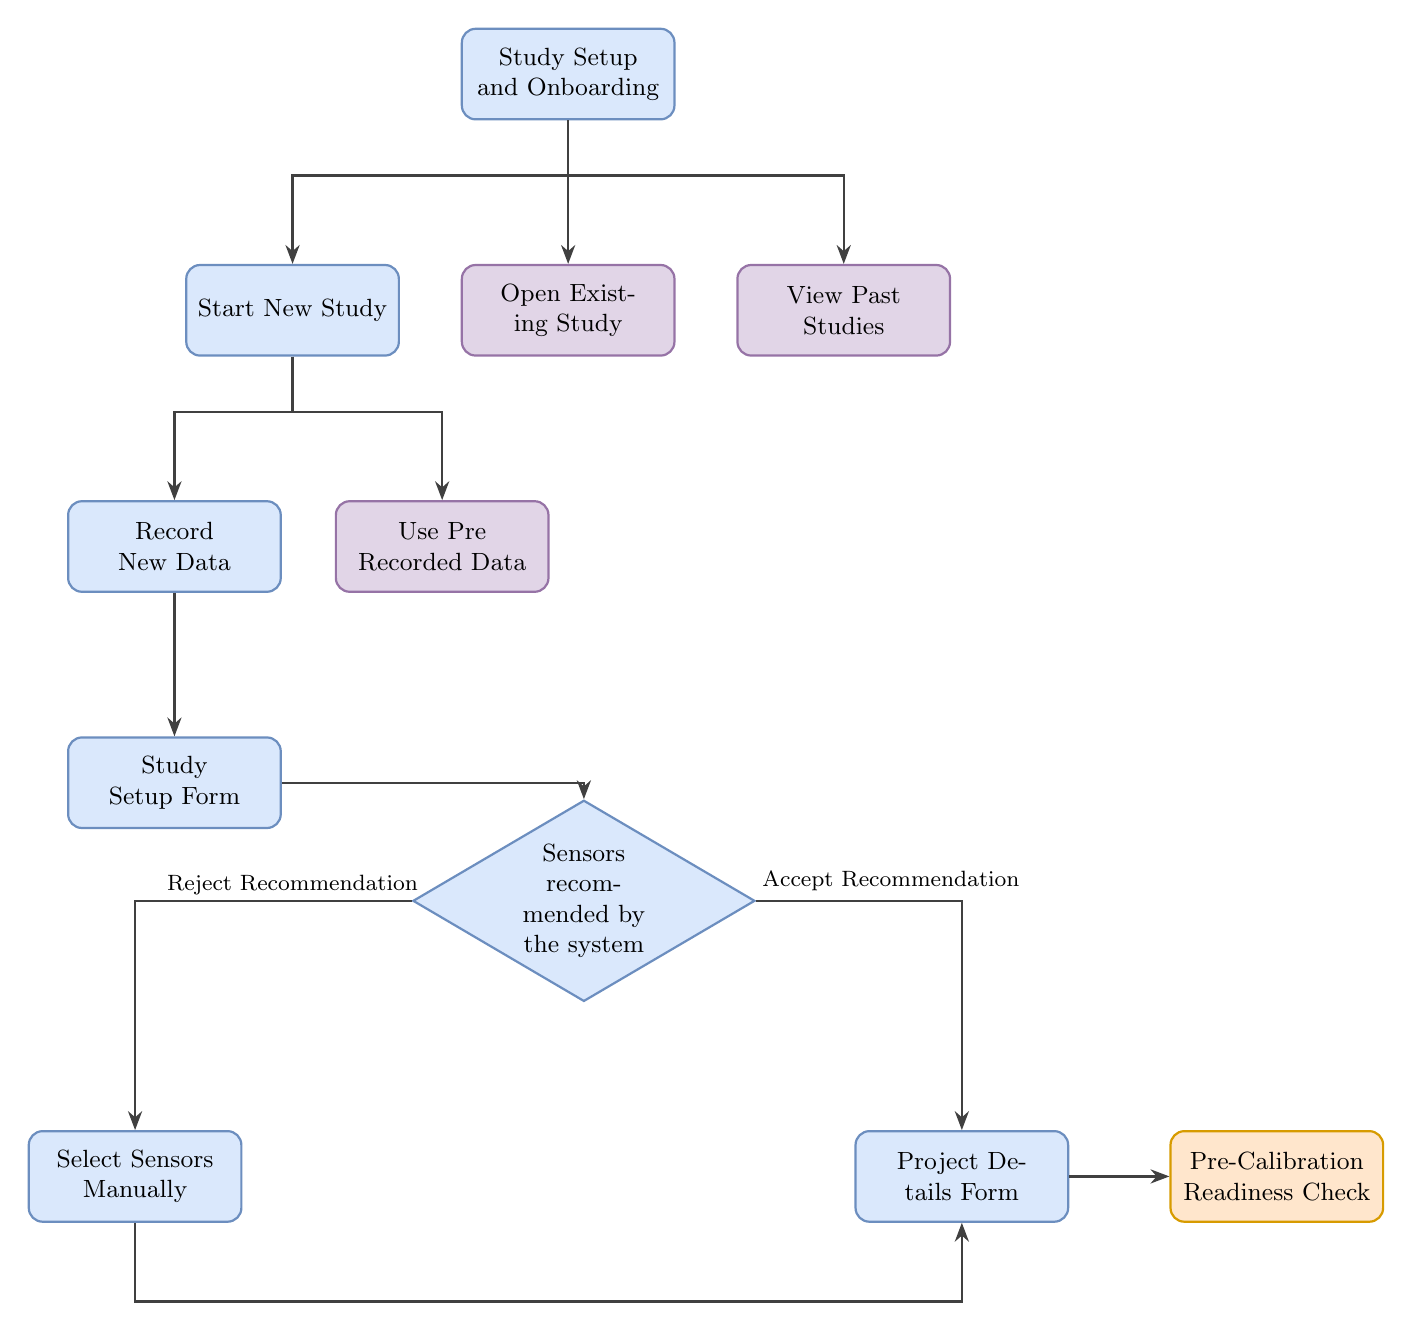
\begin{tikzpicture}[node distance=0pt]

  % ---- Nodes -------------------------------------------------------------
  \node[blue]   (root)  at (5,0)      {Study Setup and Onboarding};

  \node[blue]   (new)   at (1.5,-3)   {Start New Study};
  \node[purple] (open)  at (5,-3)     {Open Existing Study};
  \node[purple] (past)  at (8.5,-3)   {View Past Studies};

  \node[blue]   (rec)   at (0,-6)     {Record New Data};
  \node[purple] (pre)   at (3.4,-6)   {Use Pre Recorded Data};

  \node[blue]   (form)  at (0,-9)     {Study Setup Form};
  \node[bdecision](sens)at (5.2,-10.5){Sensors recommended by the system};

  \node[blue]   (manual)at (-0.5,-14) {Select Sensors Manually};
  \node[blue]   (proj)  at (10,-14)   {Project Details Form};
  \node[orange] (ready) at (14,-14)   {Pre-Calibration Readiness Check};

  % ---- Edges -------------------------------------------------------------
  % root fans out to the three top options
  \draw[flow] (root.south) -- ++(0,-0.7) -| (new.north);
  \draw[flow] (root.south) -- ++(0,-0.7) -| (open.north);
  \draw[flow] (root.south) -- ++(0,-0.7) -| (past.north);

  % start new study -> record / pre-recorded
  \draw[flow] (new.south) -- ++(0,-0.7) -| (rec.north);
  \draw[flow] (new.south) -- ++(0,-0.7) -| (pre.north);

  \draw[flow] (rec) -- (form);

  % study setup form -> recommendation decision
  \draw[flow] (form.east) -- (form.east -| sens.north) -- (sens.north);

  % decision branches: reject -> top of manual box, accept -> top of project box
  \draw[flow] (sens.west) -| (manual.north);
  \node[elabel, fill=none] at (1.5,-10.3) {Reject Recommendation};
  \draw[flow] (sens.east) -| (proj.north);
  \node[elabel, fill=none] at (9.1,-10.25) {Accept Recommendation};

  % both selection paths converge on project details, then readiness
  \draw[flow] (manual.south) |- ($(proj.south)+(0,-1)$) -- (proj.south);
  \draw[flow] (proj) -- (ready);

\end{tikzpicture}
\end{document}
